
%(BEGIN_QUESTION)
% Copyright 2005, Tony R. Kuphaldt, released under the Creative Commons Attribution License (v 1.0)
% This means you may do almost anything with this work of mine, so long as you give me proper credit

Calculus is a branch of mathematics that originated with scientific questions concerning {\it rates of change}.  The easiest rates of change for most people to understand are those dealing with time.  For example, a student watching their savings account dwindle over time as they pay for tuition and other expenses is very concerned with rates of change ({\it dollars per day} being spent).  

Rates of change are symbolically expressed in mathematical equations using the ``derivative'' notation.  For example, if the variable $S$ represents the amount of money in the student's savings account and $t$ represents time, the rate of change of dollars over time (the {\it time-derivative} of the student's account balance) would be written as $dS \over dt$.  The process of calculating this rate of change from a record of the account balance over time, or from an equation describing the balance over time, is called {\it differentiation}.

\vskip 10pt

Suppose student {\bf A} banks at Humongous Savings and Loan where daily account balances are documented to customers, while student {\bf B} banks at Isaac Newton Credit Union, where only rates of account balance {\it change} are shown in each statement.  These rates of change are always in units of dollars per day, calculated at the close of every day.  If both students began with exactly the same amount of money in each account, and withdrew exactly the same amount from each account at the same times, the two statements would compare as follows:

$$\includegraphics[width=15.5cm]{i01563x01.eps}$$

Explain how the Isaac Newton Credit Union calculates the derivative ($dS \over dt$) from the balance numbers (corresponding to $S$ in the Humongous Savings \& Loan statement), and then explain how the student who banks at Isaac Newton Credit Union could figure out how much money is in their account at any given time lacking such balance figures.

Hint: the process of calculating a variable's value from rates of change is called {\it integration} in calculus.  It is the opposite (inverse) function of differentiation.

\underbar{file i01563}
%(END_QUESTION)





%(BEGIN_ANSWER)

The Isaac Newton Credit Union differentiates $S$ by dividing the difference between consecutive balances by the number of days between those balance figures.  Differentiation is fundamentally a process of division.

To integrate the $dS\over dt$ values shown on the Credit Union's statement so as to arrive at values for $S$, we must either repeatedly add or subtract the days' rate-of-change figures, beginning with a starting balance.  Thus, integration is fundamentally a process of multiplication.

\vskip 10pt

Follow-up question: explain why a starting balance is absolutely necessary for the student banking at Isaac Newton Credit Union to know in order for them to determine their account balance at any time.  Why would it be impossible for them to figure out how much money was in their account if the only information they possessed was the $dS \over dt$ figures?

%(END_ANSWER)





%(BEGIN_NOTES)

The purpose of this question is to introduce the concept of the integral to students in a way that is familiar to them.  Hopefully the opening scenario of a dwindling savings account is something they can relate to!

Some students may ask why the differential notation $dS \over dt$ is used rather than the difference notation $\Delta S \over \Delta t$ in this example, since the rates of change are always calculated by subtraction of two data points (thus implying a $\Delta$).  Given that the function here is piecewise and not continuous, one could argue that it is not differentiable at the points of interest.  My purpose in using differential notation is to familiarize students with the concept of the derivative in the context of something they can easily relate to, even if the particular details of the application suggest a more correct notation.

Before you think to make a correction to the $dS \over dt$ figure for May 9, from \$20.81 per day to \$62.43 per day, note that this is a {\it per day} rate, and that three days span between May 9 and the next previous balance entry!

%INDEX% Mathematics, calculus: integral and derivative related to finances

%(END_NOTES)


